\documentclass[11pt,a4paper]{article}
\usepackage[utf8]{inputenc}
\usepackage[T1]{fontenc}
\usepackage{amsmath,amssymb,amsthm}
\usepackage{geometry}
\usepackage{braket}
\usepackage{tikz}
\geometry{margin=2.5cm}
\usepackage{hyperref}

\newcommand{\op}[1]{\hat{#1}}
\newcommand{\ud}{\mathrm{d}}

\title{NJSF064 --- Nuclear Physics\\[2mm]\large Lecture notes, week 2: Tensor interaction \& low-energy $NN$ scattering}
\author{Transcribed from handwritten notes}
\date{}

\begin{document}
\maketitle

\tableofcontents

%=====================================================================
\section{Deuteron --- tensor interaction}
%=====================================================================

Deuteron properties $\Rightarrow$ the $NN$ interaction must include a term
mixing states with different $L$. An interaction of the type
\[
V_1(r)+V_2(r)\,f\big(\vec\sigma^{(1)},\vec\sigma^{(2)}\big)
\]
does not mix them!

\subsection{Symmetry requirements on the \texorpdfstring{$NN$}{NN} potential}

An unknown potential has to fulfil:
\[
V=V\big(\vec r_1,\vec r_2,\vec p_1,\vec p_2,\vec\sigma^{(1)},\vec\sigma^{(2)},
\vec\tau^{(1)},\vec\tau^{(2)}\big)\equiv V(1,2),
\qquad
V(1,2)\stackrel{!}{=}V(2,1).
\]

\textbf{Translational invariance:} $\vec r_1\to\vec r_1+\vec a$,
$\vec r_2\to\vec r_2+\vec a$, $\forall\vec a$. With
\[
\vec r=\vec r_1-\vec r_2,\qquad \vec R=\tfrac12(\vec r_1+\vec r_2),\qquad
\vec p=\frac{\vec p_1-\vec p_2}{2},\qquad \vec P=\vec p_1+\vec p_2,
\]
\[
V\big(\vec r,\vec R,\vec p,\vec P,\vec\sigma^{(1)},\vec\sigma^{(2)},\vec\tau^{(1)},\vec\tau^{(2)}\big)
\stackrel{!}{=}V\big(\vec r,\vec R+\vec a,\vec p,\vec P,\dots\big)
\quad\Rightarrow\quad V \text{ cannot depend on } \vec R .
\]

\textbf{Invariance with respect to Galilean transformation:}
$\vec p_1\to\vec p_1+\vec p_0$, $\vec p_2\to\vec p_2+\vec p_0$, $\forall\vec p_0$:
\[
V\big(\vec r,\vec p,\vec P,\vec\sigma^{(1)},\vec\sigma^{(2)},\vec\tau^{(1)},\vec\tau^{(2)}\big)
\stackrel{!}{=}V\big(\vec r,\vec p,\vec P+2\vec p_0,\vec\sigma^{(1)},\vec\sigma^{(2)},\vec\tau^{(1)},\vec\tau^{(2)}\big)
\]
$\Rightarrow$ $V$ cannot depend on $\vec P$:
\[
\op V=\op V\big(\vec r,\vec p,\vec\sigma^{(1)},\vec\sigma^{(2)},\vec\tau^{(1)},\vec\tau^{(2)}\big).
\]

\textbf{Invariance with respect to parity transformation:}
\[
\op V\big(\vec r,\vec p,\vec\sigma^{(1)},\vec\sigma^{(2)},\vec\tau^{(1)},\vec\tau^{(2)}\big)
\stackrel{!}{=}\op V\big(-\vec r,-\vec p,\vec\sigma^{(1)},\vec\sigma^{(2)},\vec\tau^{(1)},\vec\tau^{(2)}\big).
\]

\subsection{Dependence on \texorpdfstring{$\vec\sigma^{(1)},\vec\sigma^{(2)}$}{sigma1, sigma2}}

Most general dependence:
\[
f\big(\vec r,\vec p,\vec\sigma^{(1)},\vec\sigma^{(2)}\big)
=\sum_{i,j=0}^{3}V_{ij}(\vec r,\vec p)\,\sigma_i^{(1)}\sigma_j^{(2)},
\qquad
\sigma_0=\mathbb 1,\quad \sigma_1=\sigma_x,\quad \sigma_2=\sigma_y,\quad \sigma_3=\sigma_z,
\]
$\Rightarrow$ terms $\sim\sigma_i^{(1,2)}$, $\ \sigma_i^{(1)}\sigma_j^{(2)}$.
More complicated terms $\sigma_i^{(\alpha)}\sigma_j^{(\alpha)}\sigma_k^{(\alpha)}$
can be reduced to $\sim\sigma_i^{(1,2)}$, $\sigma_i^{(1)}\sigma_j^{(2)}$, since
\[
\left.
\begin{aligned}
\big[\sigma_i^{(\alpha)},\sigma_j^{(\alpha)}\big]&=2i\,\varepsilon_{ijk}\,\sigma_k^{(\alpha)}\\
\big\{\sigma_i^{(\alpha)},\sigma_j^{(\alpha)}\big\}&=2\,\delta_{ij}
\end{aligned}
\right\}
\quad\Rightarrow\quad
\sigma_i^{(\alpha)}\sigma_j^{(\alpha)}=\delta_{ij}+i\,\varepsilon_{ijk}\,\sigma_k^{(\alpha)} .
\]

One can construct different operatorial terms. Important symmetries:
$\mathcal P$ --- parity, $\mathcal T$ --- time inversion ($t\to-t$).

\begin{center}
\renewcommand{\arraystretch}{1.3}
\begin{tabular}{l c c c}
\hline
\multicolumn{2}{l}{spin space} & $\mathcal P$ & $\mathcal T$ \\
\hline
scalar & $\mathbb 1$ & $+$ & $+$ \\
scalar & $\vec\sigma^{(1)}\!\cdot\vec\sigma^{(2)}$ & $+$ & $+$ \\
vector & $\vec\sigma^{(1)}\times\vec\sigma^{(2)}$ & $+$ & $+$ \\
vector & $\vec\sigma^{(1)}-\vec\sigma^{(2)}$ & $+$ & $-$ \\
vector & $\vec\sigma^{(1)}+\vec\sigma^{(2)}$ & $+$ & $-$ \\
tensor & $\big[\sigma^{(1)}\times\sigma^{(2)}\big]^2_m$ & $+$ & $+$ \\
\hline
\end{tabular}
\end{center}
with
\[
\big[\sigma^{(1)}\times\sigma^{(2)}\big]^2_m=\sum_{m_1m_2}\big(1m_1\,1m_2\,|\,2m\big)\,
\sigma^{(1)}_{1m_1}\sigma^{(2)}_{1m_2},
\]
\[
\sigma^{(\alpha)}_{10}=\sigma^{(\alpha)}_z,\quad
\sigma^{(\alpha)}_{1\pm1}=\mp\frac{1}{\sqrt2}\big(\sigma^{(\alpha)}_x\pm i\sigma^{(\alpha)}_y\big),
\quad \alpha=1,2 .
\]

Coordinate space $(\vec r,\vec p)$:
\begin{center}
\renewcommand{\arraystretch}{1.3}
\begin{tabular}{l c c c}
\hline
 & & $\mathcal P$ & $\mathcal T$ \\
\hline
scalar & $\vec r^{\,2}$ & $+$ & $+$ \\
scalar & $\vec p^{\,2}$ & $+$ & $+$ \\
scalar & $\vec r\cdot\vec p$ & $+$ & $-$ \\
vector & $\vec r$ & $-$ & $+$ \\
vector & $\vec p$ & $-$ & $-$ \\
vector & $\vec r\times\vec p$ & $+$ & $-$ \\
tensor & $\big[r_1\times p_1\big]^2_m$ & $+$ & $-$ \\
tensor & $\big[r_1\times r_1\big]^2_m$ & $+$ & $+$ \\
tensor & $\big[p_1\times p_1\big]^2_m$ & $+$ & $+$ \\
\hline
\end{tabular}
\end{center}
where $r_1$, $p_1$ denote the rank-1 (spherical) tensors built from $\vec r$, $\vec p$:
\[
\big[r_1\times r_1\big]^2_m=\sum_{m_1m_2}\big(1m_1\,1m_2\,|\,2m\big)\,r_{1m_1}r_{1m_2},
\qquad
r_{10}=z,\qquad r_{1\pm1}=\mp\frac{1}{\sqrt2}(x\pm iy).
\]

The Hamiltonian can contain only scalars. We search for vector--vector and
tensor--tensor products invariant under $\mathcal P$ and $\mathcal T$.

\textbf{Vector--vector:}
\[
(\vec r\times\vec p)\cdot\big(\vec\sigma^{(1)}+\vec\sigma^{(2)}\big)=2\,\vec L\cdot\vec S ,
\]
$(\vec r\times\vec p)\cdot\big(\vec\sigma^{(1)}-\vec\sigma^{(2)}\big)$ is not
invariant under the $1\leftrightarrow2$ exchange.

\textbf{Tensor--tensor:}
\begin{center}
\renewcommand{\arraystretch}{1.3}
\begin{tabular}{l c c c c}
\hline
 & \multicolumn{2}{c}{spin part} & \multicolumn{2}{c}{space part}\\
 & $\mathcal P$ & $\mathcal T$ & $\mathcal P$ & $\mathcal T$ \\
\hline
$\big[r_1\times r_1\big]^2\cdot\big[\sigma^{(1)}_1\times\sigma^{(2)}_1\big]^2$ & $+$ & $+$ & $+$ & $+$ \\
$\big[p_1\times p_1\big]^2\cdot\big[\sigma^{(1)}_1\times\sigma^{(2)}_1\big]^2$ & $+$ & $+$ & $+$ & $+$ \\
$\big[\sigma^{(1)}\times\sigma^{(2)}\big]^2\cdot\big[r_1\times p_1\big]^2\,(\vec r\cdot\vec p)$ & $+$ & $+$ & $+$\,$\cdot$\,$+$ & $-$\,$\cdot$\,$-$ \\
\hline
\end{tabular}
\end{center}

\subsection{The tensor operator \texorpdfstring{$\op S_{12}$}{S12}}

Tensor scalar product:
\[
A^\lambda\cdot B^\lambda=(-1)^\lambda\sqrt{2\lambda+1}\,\big[A^\lambda\times B^\lambda\big]^0_0,
\qquad
\big[r_1\times r_1\big]^2\cdot\big[\sigma^{(1)}_1\times\sigma^{(2)}_1\big]^2
=\sqrt5\,\Big[\big[r_1\times r_1\big]^2\times\big[\sigma^{(1)}\times\sigma^{(2)}\big]^2\Big]^0_0 .
\]
One can show
\[
\big[r_1\times r_1\big]^2\cdot\big[\sigma^{(1)}_1\times\sigma^{(2)}_1\big]^2
=\big(\vec\sigma^{(1)}\!\cdot\vec r\big)\big(\vec\sigma^{(2)}\!\cdot\vec r\big)
-\tfrac13\,\vec\sigma^{(1)}\!\cdot\vec\sigma^{(2)}\,r^2 .
\]

We can define the ``tensor interaction'' term
\[
\op V\equiv V_T\,\op S_{12},
\qquad
\op S_{12}=\frac{3}{r^2}\big(\vec\sigma^{(1)}\!\cdot\vec r\big)\big(\vec\sigma^{(2)}\!\cdot\vec r\big)
-\vec\sigma^{(1)}\!\cdot\vec\sigma^{(2)}
=3\big(\vec\sigma^{(1)}\!\cdot\vec n_r\big)\big(\vec\sigma^{(2)}\!\cdot\vec n_r\big)
-\vec\sigma^{(1)}\!\cdot\vec\sigma^{(2)} .
\]

\subsubsection*{Classical picture}

\begin{center}
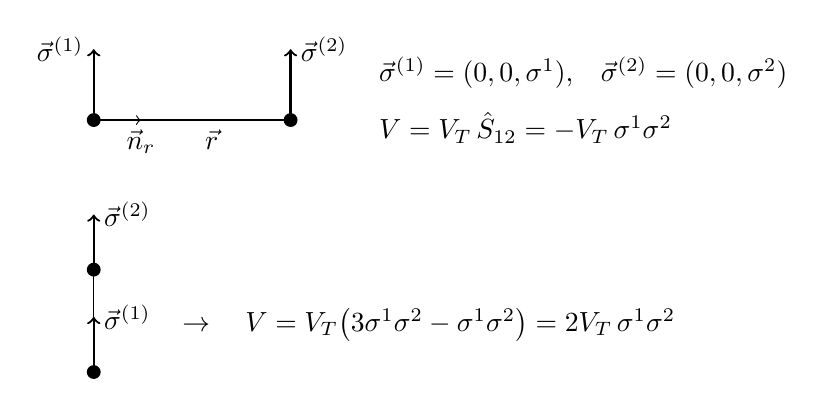
\begin{tikzpicture}[scale=1]
% spins perpendicular to r
\fill (0,0) circle (2.5pt);
\fill (2.5,0) circle (2.5pt);
\draw (0,0) -- (2.5,0);
\draw[thick,->] (0,0) -- (0,0.9) node[left]{$\vec\sigma^{(1)}$};
\draw[thick,->] (2.5,0) -- (2.5,0.9) node[right]{$\vec\sigma^{(2)}$};
\draw[->] (0,0) -- (0.6,0) node[below]{$\vec n_r$};
\node[below] at (1.5,0) {$\vec r$};
\node[right] at (3.5,0.6) {$\vec\sigma^{(1)}=(0,0,\sigma^1)$,\quad $\vec\sigma^{(2)}=(0,0,\sigma^2)$};
\node[right] at (3.5,-0.1) {$V=V_T\,\op S_{12}=-V_T\,\sigma^1\sigma^2$};
% spins parallel to r
\begin{scope}[yshift=-3.2cm]
\fill (0,0) circle (2.5pt);
\fill (0,1.3) circle (2.5pt);
\draw (0,0) -- (0,1.3);
\draw[thick,->] (0,0) -- (0,0.7) node[right]{$\vec\sigma^{(1)}$};
\draw[thick,->] (0,1.3) -- (0,2.0) node[right]{$\vec\sigma^{(2)}$};
\node[right] at (1.0,0.6) {$\to\quad V=V_T\big(3\sigma^1\sigma^2-\sigma^1\sigma^2\big)=2V_T\,\sigma^1\sigma^2$};
\end{scope}
\end{tikzpicture}
\end{center}
$\Rightarrow$ the force is not central.

\subsection{Tensor interaction in the deuteron}

Tensor interaction $\to$ mixing of states with different $L$. For the deuteron
\[
\op V=\op V_C+V_T\,\op S_{12},
\]
with $\op V_C$ the central and $V_T\op S_{12}$ the tensor part (both can depend
on spins, isospins, \dots).

Wave function:
\[
\psi_{JM}=\sum_L\psi_{LSJM},
\qquad
\psi_{LSJM}=\frac{u_L}{r}\underbrace{\sum_{m_Lm_S}\big(Lm_L\,Sm_S\,|\,JM\big)\,
Y_{Lm_L}(\theta,\varphi)\,\chi^S_{m_S}}_{\displaystyle\bar\varphi_{LSJM}}
\equiv\frac{u_L}{r}\,\bar\varphi_{LSJM} .
\]

Deuteron: $J=1$, $S=1$, $L=0,2$:
\[
\psi_{JM}=\psi_{011M}+\psi_{211M}.
\]

Schr\"odinger equation:
\begin{multline*}
\Big[-\frac{\hbar^2}{2\mu}\Big(\frac{\partial^2}{\partial r^2}+\frac2r\frac{\partial}{\partial r}
-\frac{1}{\hbar^2r^2}\op L^2\Big)+V_C+V_T\op S_{12}\Big]\big(\psi_{011M}+\psi_{211M}\big)\\
=E\big(\psi_{011M}+\psi_{211M}\big)
\qquad\Big/\ \int\!\ud\Omega\,\bar\varphi^\dagger_{011M},\ \ \int\!\ud\Omega\,\bar\varphi^\dagger_{211M}.
\end{multline*}
Projecting onto $\bar\varphi_{011M}$:
\begin{multline*}
\Big[-\frac{\hbar^2}{2\mu}\Big(\frac{\partial^2}{\partial r^2}+\frac2r\frac{\partial}{\partial r}\Big)+V_C\Big]
\frac{u_0}{r}\int\bar\varphi^\dagger_{011M}\bar\varphi_{011M}\,\ud\Omega\\
+\Big[-\frac{\hbar^2}{2\mu}\Big(\frac{\partial^2}{\partial r^2}+\frac2r\frac{\partial}{\partial r}
-\frac{2(2+1)}{r^2}\Big)+V_C\Big]\frac{u_2}{r}
\underbrace{\int\bar\varphi^\dagger_{011M}\bar\varphi_{211M}\,\ud\Omega}_{=\,0}\\
+V_T\frac{u_0}{r}\int\bar\varphi^\dagger_{011M}\op S_{12}\bar\varphi_{011M}\,\ud\Omega
+V_T\frac{u_2}{r}\int\bar\varphi^\dagger_{011M}\op S_{12}\bar\varphi_{211M}\,\ud\Omega\\
=E\Big(\frac{u_0}{r}\int\bar\varphi^\dagger_{011M}\bar\varphi_{011M}\,\ud\Omega
+\frac{u_2}{r}\underbrace{\int\bar\varphi^\dagger_{011M}\bar\varphi_{211M}\,\ud\Omega}_{=\,0}\Big).
\end{multline*}

\emph{Note:}
\begin{multline*}
\int\!\ud\Omega\,\bar\varphi^\dagger_{LSJM}\,\bar\varphi_{L'S'J'M'}\\
=\sum_{\substack{m_Lm_L'\\ m_Sm_S'}}\big(Lm_L\,Sm_S\,|\,JM\big)\big(L'm_L'\,S'm_S'\,|\,J'M'\big)
\underbrace{\int\!\ud\Omega\,Y^*_{Lm_L}(\Omega)\,Y_{L'm_L'}(\Omega)}_{\delta_{LL'}\delta_{m_Lm_L'}}
\underbrace{\chi^{S\dagger}_{m_S}\chi^{S'}_{m_S'}}_{\delta_{SS'}\delta_{m_Sm_S'}}
\end{multline*}
\[
=\delta_{LL'}\delta_{SS'}\sum_{m_Sm_L}\big(Lm_L\,Sm_S\,|\,JM\big)\big(Lm_L\,Sm_S\,|\,J'M'\big)
=\delta_{JJ'}\delta_{MM'}\delta_{LL'}\delta_{SS'} .
\]
\begin{multline*}
\Rightarrow\quad
-\frac{\hbar^2}{2\mu}\Big(\frac{\partial^2}{\partial r^2}+\frac2r\frac{\partial}{\partial r}\Big)\frac{u_0}{r}
+V_C\frac{u_0}{r}+V_T\frac{u_0}{r}\big(011M\big|\op S_{12}\big|011M\big)\\
+V_T\frac{u_2}{r}\big(011M\big|\op S_{12}\big|211M\big)=E\frac{u_0}{r},
\end{multline*}
\[
\boxed{
\begin{aligned}
-\frac{\hbar^2}{2\mu}u_0''+V_C\,u_0
&+V_T\,u_0\big(011M\big|\op S_{12}\big|011M\big)\\
&+V_T\,u_2\big(011M\big|\op S_{12}\big|211M\big)=E\,u_0
\end{aligned}
}
\]
where
\[
\big(LSJM\big|\op S_{12}\big|L'S'J'M'\big)\equiv\int\!\ud\Omega\,\bar\varphi^\dagger_{LSJM}\,\op S_{12}\,\bar\varphi_{L'S'J'M'} .
\]

In analogy,
\begin{multline*}
-\frac{\hbar^2}{2\mu}\Big(\frac{\partial^2}{\partial r^2}+\frac2r\frac{\partial}{\partial r}
-\frac{2(2+1)}{r^2}\Big)\frac{u_2}{r}+V_C\frac{u_2}{r}\\
+V_T\frac{u_0}{r}\big(211M\big|\op S_{12}\big|011M\big)
+V_T\frac{u_2}{r}\big(211M\big|\op S_{12}\big|211M\big)=E\frac{u_2}{r},
\end{multline*}
\[
\boxed{
\begin{aligned}
-\frac{\hbar^2}{2\mu}u_2''+\Big(V_C+\frac{6\hbar^2}{2\mu r^2}\Big)u_2
&+V_T\,u_0\big(211M\big|\op S_{12}\big|011M\big)\\
&+V_T\,u_2\big(211M\big|\op S_{12}\big|211M\big)=E\,u_2
\end{aligned}
}
\]

We got 2 coupled differential equations for the radial wave functions, with the
normalisation condition
\[
\int_0^\infty\big(u_0^2+u_2^2\big)\,\ud r=1 .
\]

\subsubsection*{Matrix elements of \texorpdfstring{$\op S_{12}$}{S12}}

What is $\big(LSJM\big|\op S_{12}\big|L'S'J'M'\big)$? $\op S_{12}$ is a scalar
$\to$ the matrix element cannot depend on $M$. Wigner--Eckart theorem:
\[
\big(LSJM\big|\op S_{12}\big|L'S'J'M'\big)
=\underbrace{\big(J'M'\,00\,|\,JM\big)}_{\delta_{JJ'}\delta_{MM'}}
\frac{1}{\sqrt{2J+1}}\big(LSJ\big\|\op S_{12}\big\|L'S'J'\big).
\]
One can show that
\[
\big[\op S_{12},\op S^2\big]=0
\quad\Rightarrow\quad \psi_{JM}=\psi_{JMS},
\]
i.e.\ the interaction does not mix states with $S=0$ and $S=1$:
\[
\big(LSJM\big|\op S_{12}\big|L'S'J'M'\big)=\delta_{MM'}\delta_{JJ'}\delta_{SS'}\,S_{LL'JS}.
\]
Direct evaluation leads to
\[
\big(011M\big|\op S_{12}\big|011M\big)=0,\qquad
\big(211M\big|\op S_{12}\big|011M\big)=2\sqrt2,\qquad
\big(211M\big|\op S_{12}\big|211M\big)=-2,
\]
\[
\Rightarrow\quad
\begin{aligned}
-\frac{\hbar^2}{2\mu}u_0''+V_C\,u_0+2\sqrt2\,V_T\,u_2&=E\,u_0,\\
-\frac{\hbar^2}{2\mu}u_2''+\Big(V_C+\frac{6\hbar^2}{2\mu r^2}-2V_T\Big)u_2+2\sqrt2\,V_T\,u_0&=E\,u_2 .
\end{aligned}
\]

\subsubsection*{Asymptotic solution}

For $r\gg$ range of the potential:
\[
-\frac{\hbar^2}{2\mu}\tilde u_0''=E\,\tilde u_0,\qquad
-\frac{\hbar^2}{2\mu}\tilde u_2''+\frac{6\hbar^2}{2\mu r^2}\tilde u_2=E\,\tilde u_2 .
\]
With $E=E_d<0$, $\alpha=\frac1\hbar\sqrt{2\mu|E_d|}$:
\[
\tilde u_0=A_0\,e^{-\alpha r},\qquad
\tilde u_2=A_2\,e^{-\alpha r}\Big[\frac{1}{(\alpha r)^2}+\frac{1}{\alpha r}+\frac13\Big].
\]

Finally, one can show that the deuteron wave function can be written in a
compact form:
\[
\psi_{JM}=\frac{1}{\sqrt{4\pi}}\Big(\frac{u_0}{r}+\sqrt{\tfrac18}\,\op S_{12}\,\frac{u_2}{r}\Big)\chi^1_M .
\]

%=====================================================================
\section{Proton--neutron scattering at low energies}
%=====================================================================

Phase-shift parametrisation of the scattering amplitude:
\[
f(\vartheta)=\frac1k\sum_{\ell=0}^{\infty}(2\ell+1)\,e^{i\delta_\ell}\sin\delta_\ell\,P_\ell(\cos\vartheta).
\]
For a finite-range potential, $\displaystyle\sum_{\ell=0}^{\infty}\approx\sum_{\ell=0}^{\ell_{\max}}$.

\begin{center}
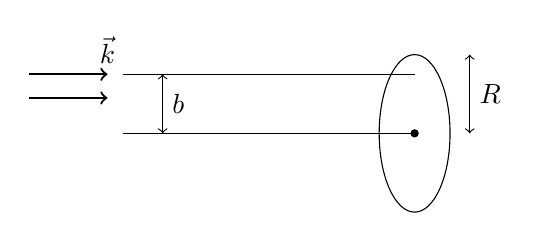
\begin{tikzpicture}[scale=1]
\draw[->,thick] (-0.4,0.75) -- (0.6,0.75) node[above]{$\vec k$};
\draw[->,thick] (-0.4,0.45) -- (0.6,0.45);
\draw (0.8,0.75) -- (4.5,0.75);
\draw (0.8,0) -- (4.5,0);
\draw[<->] (1.3,0) -- (1.3,0.75) node[midway,right]{$b$};
\draw (4.5,0) ellipse (0.45 and 1.0);
\fill (4.5,0) circle (1.5pt);
\draw[<->] (5.2,0) -- (5.2,1.0) node[midway,right]{$R$};
\end{tikzpicture}
\end{center}
\[
L_{\max}\approx R\,\hbar k,\qquad
\hbar\sqrt{\ell_{\max}(\ell_{\max}+1)}\approx R\,\hbar k
\quad\Rightarrow\quad \ell_{\max}\approx Rk .
\]
For small enough energies ($Rk\ll1$), $\ell_{\max}=0$ $\to$ only the $s$-wave
contributes to $f$:
\[
f(\vartheta)\approx\frac1k\,e^{i\delta_0}\sin\delta_0,
\qquad \delta_0 \text{ --- $s$-wave phase shift.}
\]

We define the ``scattering length'' for $E\to0$ ($k\to0$, $\delta_0\to0$):
\[
a\equiv\lim_{k\to0}\Big[-\frac{\sin\delta_0}{k}\Big]
\quad\Rightarrow\quad
\sigma\approx\int\frac{\ud\sigma}{\ud\Omega}\,\ud\Omega=\int|f|^2\,\ud\Omega
=\frac{4\pi}{k^2}\sin^2\delta_0=4\pi a^2 .
\]

\subsection{Scattering length in a simple model}

We can determine the scattering length for $p$--$n$ scattering in a simple
square-well model ($m$ is the nucleon mass, $2\mu=m$):

\begin{center}
\begin{tikzpicture}[scale=1]
\draw[->] (-0.3,1.3) -- (4.0,1.3) node[right]{$r$};
\draw[->] (0,-1.5) -- (0,1.8);
\draw[thick] (0,1.3) -- (0,-1) -- (1.6,-1) -- (1.6,1.3);
\draw[dashed] (0,-1) -- (-0.2,-1) node[left]{$-V_0$};
\node[above] at (1.6,1.3) {$R$};
\node[right] at (4.6,0.2) {$V_0=34\ \text{MeV}$};
\end{tikzpicture}
\end{center}
\[
r\le R:\quad u''+\frac{m}{\hbar^2}(E+V_0)\,u=0,
\qquad\qquad
r\ge R:\quad u''+\frac{m}{\hbar^2}E\,u=0 .
\]
For
\[
r\le R:\quad u(r)=A\sin Kr,\qquad K=\sqrt{\frac{m(E+V_0)}{\hbar^2}},
\]
\[
r\ge R:\quad u(r)=B\sin(kr+\delta),\qquad k=\sqrt{\frac{mE}{\hbar^2}} .
\]
Matching $u'/u$ at $r=R$:
\[
\frac{AK\cos(KR)}{A\sin(KR)}=\frac{Bk\cos(kR+\delta)}{B\sin(kR+\delta)}
\quad\Rightarrow\quad
K\tan(kR+\delta)=k\tan(KR),
\]
\[
K\,\frac{\tan(kR)+\tan\delta}{1-\tan(kR)\tan\delta}=k\tan(KR),
\]
\[
K\big(\tan(kR)+\tan\delta\big)=k\tan(KR)-k\tan(KR)\tan(kR)\tan\delta,
\]
\[
\tan\delta=\frac{k\tan(KR)-K\tan(kR)}{K+k\tan(KR)\tan(kR)}
=\frac{k\Big[\tan(KR)-KR\,\dfrac{\tan(kR)}{kR}\Big]}{K+k\tan(KR)\tan(kR)} .
\]

For small $E$ ($k$):
\[
\delta\approx\frac{k\big[\tan(KR)-KR\big]}{K}=kR\Big(\frac{\tan KR}{KR}-1\Big).
\]
Let us use $V_0=34$~MeV: $K=\frac{\sqrt{mV_0}}{\hbar}\doteq0.91\ \text{fm}^{-1}$.
Scattering length:
\[
a=\lim_{k\to0}\Big[-\frac{\sin\delta}{k}\Big]\approx-\frac{\delta}{k},
\qquad
a\approx R\Big[1-\frac{\tan(KR)}{KR}\Big],
\qquad \sigma=4\pi a^2 .
\]

\begin{center}
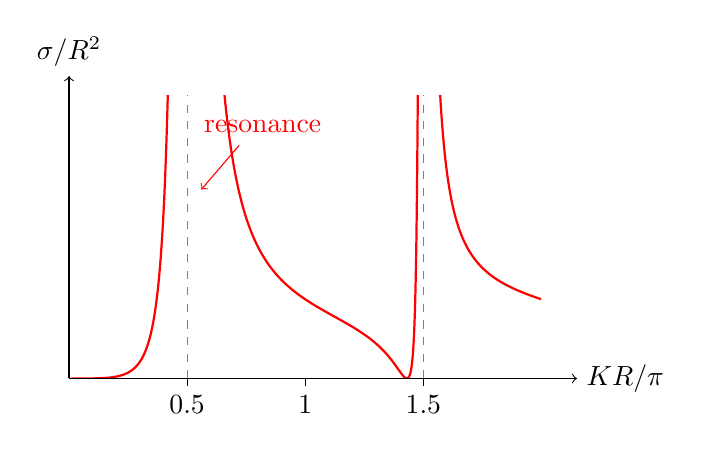
\begin{tikzpicture}[xscale=3,yscale=0.08]
\begin{scope}
\clip (0,0) rectangle (2,45);
\draw[red,thick,domain=0.01:0.497,samples=120,smooth,variable=\t]
  plot ({\t},{4*pi*(min(2.5,abs(1-tan(pi*\t r)/(pi*\t))))^2});
\draw[red,thick,domain=0.503:1.497,samples=200,smooth,variable=\t]
  plot ({\t},{4*pi*(min(2.5,abs(1-tan(pi*\t r)/(pi*\t))))^2});
\draw[red,thick,domain=1.503:2,samples=120,smooth,variable=\t]
  plot ({\t},{4*pi*(min(2.5,abs(1-tan(pi*\t r)/(pi*\t))))^2});
\end{scope}
\draw[->] (0,0) -- (2.15,0) node[right]{$KR/\pi$};
\draw[->] (0,0) -- (0,48) node[above]{$\sigma/R^2$};
\foreach \x in {0.5,1,1.5} \draw (\x,0) -- (\x,-1.2) node[below]{$\x$};
\draw[dashed,gray] (0.5,0) -- (0.5,45);
\draw[dashed,gray] (1.5,0) -- (1.5,45);
\node[red] at (0.82,40) {resonance};
\draw[red,->] (0.72,37) -- (0.56,30);
\end{tikzpicture}
\end{center}
which for $R=2.1$~fm gives $a\simeq5.2$~fm and $\sigma\simeq3.4$~b.
However, the experimental value is $\sigma^{\rm exp}\simeq20$~b.

\subsection{Spin dependence: singlet and triplet scattering}

Idea of Wigner $\to$ spin dependence of the $pn$ force. We have 2 possibilities:
$S=0$ (singlet) and $S=1$ (triplet),
\[
\sigma=\tfrac34\,\sigma_t+\tfrac14\,\sigma_s
\qquad(\sigma_t \text{ --- triplet},\ \sigma_s \text{ --- singlet}).
\]

Further measurements: scattering on ortho- and para-H$_2$ (nuclear spins):
\begin{center}
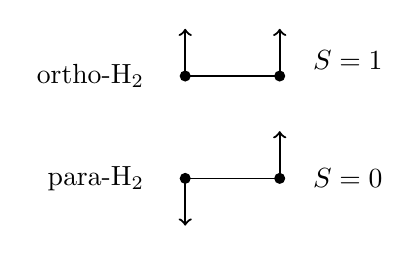
\begin{tikzpicture}[scale=1]
\node[left] at (-0.4,0.3) {ortho-H$_2$};
\fill (0,0.3) circle (2pt); \fill (1.2,0.3) circle (2pt);
\draw (0,0.3) -- (1.2,0.3);
\draw[thick,->] (0,0.3) -- (0,0.9);
\draw[thick,->] (1.2,0.3) -- (1.2,0.9);
\node[right] at (1.5,0.5) {$S=1$};
\node[left] at (-0.4,-1.0) {para-H$_2$};
\fill (0,-1.0) circle (2pt); \fill (1.2,-1.0) circle (2pt);
\draw (0,-1.0) -- (1.2,-1.0);
\draw[thick,->] (0,-1.0) -- (0,-1.6);
\draw[thick,->] (1.2,-1.0) -- (1.2,-0.4);
\node[right] at (1.5,-1.0) {$S=0$};
\end{tikzpicture}
\end{center}

$pn$ scattering:
\[
\sigma=\tfrac34\,\sigma_t+\tfrac14\,\sigma_s,\qquad
\sigma_t=4\pi a_t^2,\qquad \sigma_s=4\pi a_s^2,
\]
$a_t$, $a_s$ --- scattering lengths for triplet and singlet.

$n$--H$_2$ scattering:
\[
\sigma_{\rm para}=\pi\big(3a_t+a_s\big)^2,\qquad
\sigma_{\rm ortho}=\pi\Big[\big(3a_t+a_s\big)^2+2\big(a_t-a_s\big)^2\Big].
\]
One can also notice that $\sigma_{\rm ortho}\gg\sigma_{\rm para}$.
$\Rightarrow$ experimental values
\[
a_t\simeq5.4\ \text{fm},\qquad a_s\simeq-23.7\ \text{fm},
\]
\[
\sigma_t=4\pi a_t^2\simeq3.7\ \text{b}\qquad[1\,\text{b}=100\ \text{fm}^2],
\qquad
\sigma_s=4\pi a_s^2\simeq70.6\ \text{b},
\qquad
\sigma\simeq20\ \text{b}.
\]
Note that $\sigma_t\simeq3.7$~b is not so far from our simple estimate based on
the square-well potential.

\subsection{Effective-range expansion}

One can show that the cross section for low-energy scattering up to
$\approx10$~MeV can be described by the formula
\[
\sigma=\frac{4\pi a^2}{k^2a^2+\big(1-\tfrac12\,a\,k^2\,r\big)^2},
\]
i.e.\ we have 2 phenomenological parameters:
\begin{itemize}
\item $a$ --- scattering length,
\item $r$ --- so-called effective range.
\end{itemize}
Such a description is \textbf{not} sensitive to the shape of the potential.

The spin dependence of the $NN$ force moreover implies a different potential in
the singlet and triplet state. Therefore we have 4 parameters
$(a_s,r_s,a_t,r_t)$ and
\[
\sigma=\tfrac34\,\sigma_t+\tfrac14\,\sigma_s
=\frac34\,\frac{4\pi a_t^2}{a_t^2k^2+\big(1-\tfrac12a_tr_tk^2\big)^2}
+\frac14\,\frac{4\pi a_s^2}{a_s^2k^2+\big(1-\tfrac12a_sr_sk^2\big)^2}.
\]

\subsection{\texorpdfstring{$p$--$p$}{p-p} scattering}

$p$--$p$ scattering is more complicated due to the long-range Coulomb
interaction, and the particles are identical:
\[
\frac{\ud\sigma}{\ud\Omega}\sim\big|f(\vartheta,\varphi)+f(\pi-\vartheta,\pi+\varphi)\big|^2 .
\]

\begin{center}
\begin{tikzpicture}[scale=1]
% direct
\draw (0,1.5) -- (1.8,1.5);
\draw[->] (1.8,1.5) -- (2.6,1.95);
\draw (2.6,1.95) -- (3.4,2.4);
\draw (4.0,1.6) -- (2.2,1.6);
\draw[->] (2.2,1.6) -- (1.5,0.95);
\draw (1.5,0.95) -- (0.8,0.3);
% exchange
\begin{scope}[xshift=5cm]
\draw (0,1.5) -- (1.9,1.5) .. controls (2.3,1.5) and (2.2,1.1) .. (1.7,0.8);
\draw[->] (1.7,0.8) -- (1.2,0.45);
\draw (1.2,0.45) -- (0.6,0.1);
\draw (4.2,1.5) -- (2.5,1.5) .. controls (2.1,1.5) and (2.4,1.9) .. (2.8,2.1);
\draw[->] (2.8,2.1) -- (3.2,2.35);
\draw (3.2,2.35) -- (3.6,2.6);
\end{scope}
\end{tikzpicture}
\end{center}

Spin parts:
\[
L=0,2,4,\dots:\ \chi^0,\qquad\qquad L=1,3,5,\dots:\ \chi^1 .
\]

\[
f=f^C+f^N\qquad(f^C \text{ --- Coulomb},\ f^N \text{ --- nuclear}),
\]
\[
\frac{\ud\sigma}{\ud\Omega}=\Big(\frac{\ud\sigma}{\ud\Omega}\Big)_C
+\Big(\frac{\ud\sigma}{\ud\Omega}\Big)_N
+\Big(\frac{\ud\sigma}{\ud\Omega}\Big)_{CN}
\quad(\to \text{interference term}),
\]
\[
\Big(\frac{\ud\sigma}{\ud\Omega}\Big)_N\approx\frac{\sin^2\delta_0}{k^2}
\qquad\text{for small energies.}
\]

\subsection{Higher partial waves}

To get information about the details of the potential, we have to include
higher partial waves, $\ell>0$. Starting from
\[
f(\vartheta)=\frac1k\sum_{\ell=0}^{\infty}(2\ell+1)\,e^{i\delta_\ell}\sin\delta_\ell\,P_\ell(\cos\vartheta)
\]
and keeping $\ell=0,1$:
\[
f(\vartheta)=\frac1k\,e^{i\delta_0}\sin\delta_0+\frac1k\,3\,e^{i\delta_1}\sin\delta_1\cos\vartheta ,
\]
\[
|f(\vartheta)|^2=|f_0+f_1|^2=|f_0|^2+|f_1|^2+2\,\mathrm{Re}\big(f_0^*f_1\big),
\]
\[
f_0^*f_1=\frac{1}{k^2}\,3\,e^{i(\delta_1-\delta_0)}\sin\delta_0\sin\delta_1\cos\vartheta,
\qquad
\mathrm{Re}\big(f_0^*f_1\big)=\frac{1}{k^2}\,3\cos(\delta_1-\delta_0)\sin\delta_0\sin\delta_1\cos\vartheta,
\]
\[
\frac{\ud\sigma}{\ud\Omega}=\frac{1}{k^2}\Big(
\underbrace{\sin^2\delta_0}_{\ell=0}+\underbrace{9\sin^2\delta_1\cos^2\vartheta}_{\ell=1}
+\underbrace{6\cos(\delta_1-\delta_0)\sin\delta_0\sin\delta_1\cos\vartheta}_{\text{interf.\ term}}\Big).
\]

It makes sense to include data up to $\approx280$~MeV (in the lab, i.e.\
$140$~MeV in the CM) for elastic scattering; above that, production of $\pi$
sets in.

\end{document}
